\documentclass{beamer}
\usetheme{Madrid}
\usepackage[spanish]{babel}
\usecolortheme{default}
\usepackage{emoji}
\usepackage[most]{tcolorbox}
\usepackage{listings}
\usepackage{xcolor}
\usepackage{graphicx}
\usepackage{algorithm}
\usepackage{algpseudocode}
\usepackage{float}
\usepackage{mathtools}
\usepackage{hyperref}
\makeatletter
\newcases{centercases}{\quad}
  {\hfil$\m@th\displaystyle{##}$\hfil}
  {$\m@th\displaystyle{##}$\hfil}{\lbrace}{.}
\makeatother

\usepackage{comment}
\usepackage{minted}

% Define Python syntax highlighting
\lstdefinestyle{pythonstyle}{
    language=Python,
    basicstyle=\ttfamily\tiny,
    keywordstyle=\color{blue},
    commentstyle=\color{gray},
    stringstyle=\color{red},
    numbers=left,
    numberstyle=\tiny\color{gray},
    stepnumber=1,
    showstringspaces=false,
    frame=none,
    breaklines=true,
    numbersep=4pt, % Reduce space between numbers and text
    xleftmargin=10pt % Reduce left margin for compactness
}






%Information to be included in the title page:
\title[Virtualización] %optional
{Virtualización}

\subtitle{MISUM}

\author[José A.] % (optional, for multiple authors)
{José Antonio Hernández López\inst{1}}

\institute[UMU] % (optional)
{
  \inst{1}%
  Departamento de Informática y Sistemas\\
  Universidad de Murcia
}

%\date[VLC 2021] % (optional)
%{Very Large Conference, April 2021}



%\logo{\includegraphics[height=1cm]{overleaf-logo}}
\begin{document}

\frame{\titlepage}

\begin{frame}
\frametitle{Índice}
\tableofcontents
\end{frame}

\section{Virtualización}

\subsection{Definición}

\begin{frame}{Virtualización}


\begin{block}{Definición}
Virtualización es una tecnología que crea versiones virtuales de recursos computacionales (servidores, redes, almacenamiento, etc.). 

Permite que haya múltiples instancias lógicas (algunas veces llamadas máquinas virtuales o contenedores, dependiendo del enfoque) ejecutándose en una máquina física.
\end{block}
%Virtualization is a technology that creates a virtual (rather than physical) version of computing resources. It allows multiple logical instances (called virtual machines or containers, depending on the approach) to run on a single physical system by abstracting and sharing its hardware/software resources.
\pause
Tipos de virtualización:

\begin{itemize}
    \item \textbf{Virtualización de hardware}
    \item \textbf{Virtualización de sistema operativo (contenedorización)}
    \item Virtualización de redes
    \item Virtualización de almacenamiento
    \item ...
    \end{itemize}

\end{frame}

\subsection{Tipos}

\begin{frame}{Virtualización de hardware}

\begin{block}{Definición}
La virtualización de hardware es el proceso de crear una o más máquinas virtuales (MV) en un servidor físico mediante la abstracción de sus recursos de hardware (CPU, memoria, almacenamiento, red).

\vspace{5pt}

MV $=$ SO con su kernel, drivers, aplicaciones, programas

\end{block}

\pause

\begin{itemize}
    \item Cada MV se comporta como un ordenador real con su propio sistema operativo, aplicaciones y hardware virtual (CPU, disco, tarjeta de red)

    \pause
    
    \item La idea principal es usar un \textit{hypervisor} que actúa como una capa entre el hardware físico y las máquinas virtuales

    \pause
    
    \item Es la base del \textit{cloud computing}

    \pause
    
    \item Ejemplos: Xen, KVM, \textbf{Oracle VirtualBox}, VMWare, Hyper-V
\end{itemize}
    
\end{frame}

\begin{frame}{Virtualización de hardware}

Conceptos clave:

\begin{itemize}
    \item \textbf{Host}: servidor o máquina física donde se ejecuta la virtualización.
    \item \textbf{Guest}: la máquina virtual que se ejecuta dentro del host.
    \item \textbf{Hypervisor}: software que permite la virtualización. Reserva recursos y asegura aislamiento entre guests.
\end{itemize}

\pause 

\vspace{10pt}

Tips de virtualización de hardware:

\begin{figure}
    \centering
    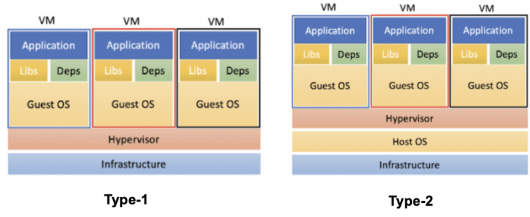
\includegraphics[width=0.5\linewidth]{hypervisor.png}
\end{figure}

\end{frame}

\begin{frame}{Virtualización de sistema operativo (contenedorización)}



\begin{block}{Definición}
La virtualización del sistema operativo es una tecnología que permite que múltiples entornos de espacio de usuario aislados (llamados contenedores) se ejecuten sobre un único núcleo (kernel) del sistema operativo.

\vspace{5pt}
Contendor $=$ proceso aislado que contiene todos los ficheros necesarios para ejecutarse.
\end{block}

\pause

{\scriptsize
Contenedores vs MVs:
\begin{itemize}
    \item Kernel: Los contenedores no incluyen kernel y usan el kernel del host. Las MVs son SOs completos

    \pause
    
    \item Arranque: Los contenedores son más rápidos en arrancar. Arrancar una MV es como arrancar un ordenador

    \pause
    
    
    \item Aislamiento: El aislamiento entre MVs es mayor que entre contenedores. Los contenedores comparten el mismo kernel

    \pause
    
    
    \item Flexibilidad: Las MVs son más flexibles. Solo puedes ejecutar contenedores si encajan con el kernel del host

    \pause

    
    \item Uso de recursos: los contendores son procesos + librerías. Las MVs son RAM + CPU + SO
\end{itemize}}
    
\end{frame}

\begin{frame}{Virtualización de sistema operativo (contenedorización)}

La tecnología más famosa que permite esta virtualización es \textbf{Docker}.

\begin{figure}
    \centering
    
\includegraphics[width=0.6\linewidth]{docker.png}
\end{figure}
    
\end{frame}

\begin{comment}

\begin{frame}{Virtualización de redes}

\begin{block}{Definición}
La virtualización de redes consiste en abstraer los recursos físicos de red (switches, routers, firewalls, balanceadores, etc.) y presentarlos como recursos lógicos/virtuales, que pueden gestionarse de forma centralizada y programable mediante software.

Es decir, se crean \textbf{redes virtuales} que funcionan sobre la infraestructura física existente, de manera similar a cómo las máquinas virtuales funcionan sobre un servidor físico.
\end{block}

\begin{itemize}
    %\item Abstracción: separa la capa de control (gestión del tráfico) de la capa de datos (tráfico real).

 \item Aislamiento: permite crear múltiples redes virtuales sobre la misma infraestructura física.

 \item Automatización: la configuración de red se gestiona por software.

\item Escalabilidad: es más fácil crear, eliminar o modificar redes para distintos entornos (dev, test, producción).
\end{itemize}
    
\end{frame}

\begin{frame}{Virtualización de redes}

Conceptos clave:

\begin{itemize}
    \item Redes definidas por software (SDN)
    \item Virtualización de funciones de red (NFV)
\end{itemize}
    
\end{frame}

\begin{frame}{Virtualización de redes: Redes definidas por software}

\begin{block}{Definición}
Son una forma de diseñar y gestionar redes donde el control de la red está separado de los dispositivos que mueven el tráfico.
\end{block}

En redes tradicionales:

\begin{itemize}
    \item Plano de control: decide dónde enviar los paquetes (tablas de enrutamiento, ACL, configuraciones de VLAN).
    
    \item Plano de datos: reenvía los paquetes a velocidad de línea.
\end{itemize}

En SDN, estos se dividen:

\begin{itemize}
    \item El plano de datos permanece en los switches/routers 

    \item El plano de control se extrae y se centraliza en un controlador de software (un cerebro que programa los dispositivos mediante API/protocolos)
\end{itemize}
    
\end{frame}


\end{comment}

\subsection{Virtualización y DevOps}

\begin{frame}{Aislamiento y reproducibilidad}

DevOps requiere entornos consistentes en desarrollo, pruebas y producción.

\begin{itemize}
    \item \textbf{Máquinas virtuales}: cada una con su propio sistema operativo $\rightarrow$ aislamiento robusto para probar diferentes plataformas (Linux, Windows)
    \item \textbf{Contenedores}: el mismo kernel del host, pero con espacio de usuario aislado $\rightarrow$ entornos ligeros y reproducibles
\end{itemize}


\begin{tcolorbox}[colback=red!5!white,colframe=red!75!black]
    \textbf{Soluciona el problema "no funciona en mi PC"}
\end{tcolorbox}
    
\end{frame}

\begin{frame}{Infraestructura como código y automatización}

Hay tecnologías que permiten definir MVs/contenedores como un archivo de código (\textbf{IaC}) y lanzarlos con un simple comando (\textbf{automatización}). Esos comandos pueden ser llamados en pipelines CI/CD.

\begin{itemize}
    \item Máquinas virtuales: Vagrant permite describir (\texttt{Vagrantfile}) y lanzar (\texttt{vagrant up}) muy fácilmente MVs.
    \item Contenedores: Docker permite describir (\texttt{Dockerfile} o \texttt{docker-compose.yml}) y lanzar (\texttt{docker-compose up}) muy fácilmente contenedores.
\end{itemize}

    
\end{frame}

\begin{frame}[fragile]{Infraestructura como código y automatización}

Ejemplo de Vagrant en Jenkins CI/CD pipeline.

\begin{minted}[fontsize=\scriptsize]{python}
pipeline {
  ...
  stages {
    stage('Checkout') {
      steps { checkout scm }
    }

    stage('Up VMs') {
      steps {
        sh 'vagrant up '
      }
    }

    stage('Run Tests') {
      steps {
        sh 'vagrant ssh -c "cd /vagrant && ./scripts/run_tests.sh"'
      }
    }
  }
  ...
}

\end{minted}
    
\end{frame}



\section{Vagrant}

\begin{frame}{Vagrant}
\begin{block}{Vagrant}
Vagrant es una herramienta OS de software (de HashiCorp) que sirve para crear y gestionar entornos de desarrollo virtualizados de forma sencilla y reproducible.
\end{block}

\begin{itemize}
    \item Automatiza la creación de MV con VirtualBox, VMWare y Hyper-V
    \item Se integra bien con herramientas de gestión de la configuración como Ansible
    \item Funciona en Linux, Windows, MacOS
\end{itemize}

\begin{figure}
    \centering
    
\includegraphics[width=0.5\linewidth]{vagrant.png}
\end{figure}

\end{frame}

\begin{frame}{Vagrant}

¿Por qué usar Vagrant?

\begin{itemize}
    \item Crear nuevas máquinas virtuales de forma rápida y sencilla (\texttt{vagrant up})
    \item Reproducibilidad
    \item Entorno idéntico en el desarrollo y la producción
    \item Portabilidad
    \begin{itemize}
        \item Adiós \texttt{.ova} de 4GB
        \item Solo \texttt{git clone} y \texttt{vagrant up}
    \end{itemize}

\end{itemize}
    
\end{frame}

\begin{frame}{Vagrant}

Componentes clave:

\begin{itemize}
    \item Archivo \texttt{Vagrantfile}: archivo de configuración de Vagrant que indica \textit{qué quiero y cómo lo quiero}
    \item Box: plantilla base de la MV
    \item Comandos: crear, iniciar, detener y gestionar MVs
\end{itemize}
    
\end{frame}

\begin{frame}[fragile]{Vagrant}
El fichero \texttt{Vagrantfile}:
\begin{itemize}
    \item Se suele encontrar en la raíz de repositorio
    \item Describe la configuración de la MV
    \item Define los recursos
    \item Escrito en Ruby
\end{itemize}

\vspace{5pt}
\begin{minted}[fontsize=\scriptsize]{ruby}
Vagrant.configure("2") do |config|
  config.vm.box = "ubuntu/focal64"   # box base
  config.vm.network "forwarded_port", guest: 80, host: 8080 # host:8080 -> guest:80  
  config.vm.provider "virtualbox" do |vb|
    vb.memory = "1024"   # RAM asignada
  end
end

\end{minted}
\end{frame}

\begin{frame}{Vagrant} 

Una box:

\begin{itemize}
    \item Es la imagen base de la máquina virtual
    \item Similar a una "plantilla": contiene un sistema operativo preconfigurado (ej. Ubuntu, CentOS, Debian, ...)
    \item Se suele descargar de Vagrant Cloud\footnote{\url{https://portal.cloud.hashicorp.com/vagrant/discover}}
    \item Ejemplo \texttt{config.vm.box = ''ubuntu/focal64''} es la box oficial de Ubuntu 20.04
\end{itemize}

\end{frame}

\begin{frame}{Vagrant}

Comandos:

\begin{itemize}
    \item \texttt{vagrant init}: inicializa un Vagrantfile
    \item \texttt{vagrant up}: crea y arranca una máquina virtual
    \item \texttt{vagrant ssh}: acceso a la máquina virtual
    \item \texttt{vagrant halt}: apaga la máquina virtual
    \item \texttt{vagrant destroy}: elimina la máquiva virtual

\end{itemize}
    
\end{frame}

\begin{frame}[fragile]{Vagrant}

Ejemplo de uso de Vagrant (ejemplo de juguete Apache web server):

\begin{enumerate}
    \item Clonamos repositorio \texttt{git clone repo \&\& cd repo}. El repositorio debe tener un \texttt{Vagrantfile}.
    \begin{minted}[fontsize=\scriptsize]{ruby}
Vagrant.configure("2") do |config|
  config.vm.box = "ubuntu/focal64"
  config.vm.network "forwarded_port", guest: 80, host: 8080
  config.vm.synced_folder "./html", "/var/www/html"
  config.vm.provision "shell", inline: <<-SHELL
    apt-get update
    apt-get install -y apache2
    systemctl enable apache2
    systemctl start apache2
  SHELL
end
\end{minted}
    
    \item Se ejecuta \texttt{vagrant up} que hará lo siguiente:
    \begin{itemize}
        \item Vagrant descargará la box (\texttt{ubuntu/focal64}) si no la tienes
        \item Creará la máquina en VirtualBox (o en el provider que esté)
        \item Instalará Apache dentro de la MV
        \item Montará tu carpeta \texttt{html/} local en \texttt{/var/www/html} de la MV

    \end{itemize}
    \item Yendo a la dirección \texttt{http://localhost:8080} se verá el contenido de la carpeta \texttt{html/} (proyecto web)
\end{enumerate}
    
\end{frame}




\section{Docker}

\begin{frame}{Docker}

\begin{block}{Docker}
Docker es una plataforma de código abierto que le permite crear, empaquetar y ejecutar aplicaciones en entornos aislados llamados contenedores (virtualización de sistema operativo).    
\end{block}

{\scriptsize\begin{itemize}
    \item Se apoya en namespaces de Linux para aislar recursos entre contenedores. Cada contendor tiene su propio árbol de procesos, pila de red, sistema de ficheros, etc.
    
    \item Usa \texttt{cgroups} para limitar recursos (CPU, RAM, disco) y asegurar un reparto controlado y justo de recursos entre contenedores
    \item Todo corre sobre un único kernel compartido de Linux
    \item Funciona en Windows porque Docker (Desktop) instala y gestiona automáticamente una pequeña máquina virtual Linux en segundo plano
\end{itemize}}

\begin{figure}
    \centering
    
\includegraphics[width=0.2\linewidth]{docker.png}
\end{figure}
    
\end{frame}

\begin{frame}{Docker}
\begin{figure}
    \centering
    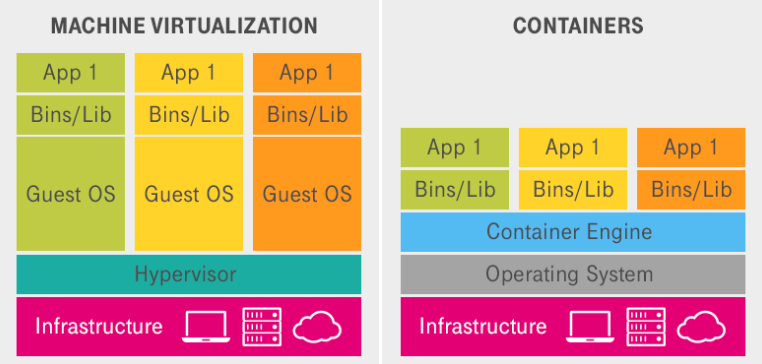
\includegraphics[width=0.8\linewidth]{vmvscontainer.png}
\end{figure}
\end{frame}

\begin{frame}{Docker}

Principales componentes de Docker:
\begin{itemize}
    \item Docker client: Es la interfaz con la que se interactúa. Se comunica con el daemon usando la API REST de Docker.
    \item Docker engine: está formado por el Docker daemon y la Docker API:
        \begin{itemize}
            \item Docker daemon: proceso en segundo plano que escucha peticiones del Docker API, construye imágenes, arranca y detiene contendores, gestiona redes, volúmenes, \texttt{cgroups}, etc.
            \item Docker API: Interfaz REST que permite que clientes, herramientas externas o interfaces gráficas hablen con el daemon
        \end{itemize}
        
    \item Docker image: plantillas inmutables que contienen: el sistema de archivos necesario (librerías, binarios, dependencias, etc.), metadatos (variables de entorno, puertos, comandos por defecto), e instrucciones de construcción.
    \item Docker container: instancias en ejecución de imágenes
    \item Docker Hub: registro público de imágenes
    \item Docker Networking \& Volumes: para gestionar redes entre contenedores y persistencia
\end{itemize}
    
\end{frame}

\begin{frame}{Docker}

Ecosistemas adicional que no son principales:
\begin{itemize}
    \item Docker compose: Orquestar varios contenedores definidos en docker-compose.yml. Ideal para desarrollo local.
    \item Docker Swarm: Orquestación nativa de clústeres de Docker (antes de Kubernetes).
    \item Docker Desktop: GUI + integración con WSL 2 (en Windows/Mac) para ejecutar contenedores Linux fácilmente.
\end{itemize}
    
\end{frame}

\begin{frame}{Docker}

Ejemplo, el usuario ejecuta:

\begin{center}
    \texttt{docker run -d -p 8080:80 nginx}

\end{center}
desde la terminal (bash, PowerShell, etc.).

\end{frame}


\begin{frame}{Docker}
\begin{itemize}
  \item \textbf{Interacción del usuario:}  
  Tras ejecutar el comando, el \textbf{Docker Client} (CLI) envia la orden.

  \item \textbf{Comunicación con el daemon:}  
  El cliente envía la orden al \textbf{Docker Daemon} a través de la \textbf{Docker API} (socket Unix o TCP).

  \item \textbf{Resolución de la imagen:}  
  El daemon comprueba si la imagen \texttt{nginx} está disponible localmente.  
  Si no, la descarga desde el \textbf{registro de imágenes} (Docker Hub) y la guarda en el almacén local.

  \item \textbf{Creación del contenedor:}  
  El daemon crea la instancia:
  \begin{itemize}
    \item Monta las capas de la imagen.
    \item Configura \textbf{namespaces} para aislamiento.
    \item Crea un \textbf{cgroup} para controlar recursos.
    \item Configura red y mapeo de puertos (8080 → 80).
  \end{itemize}

  \item \textbf{Ejecución del proceso:}  
  El daemon lanza el proceso principal de la imagen (en este caso, \texttt{nginx}), dentro de los namespaces y cgroup creados.  
  → El kernel ejecuta el proceso aislado.

  \item \textbf{Exposición del servicio:}  
  Gracias al mapeo de puertos, las peticiones a \texttt{localhost:8080} se redirigen al puerto 80 del contenedor.
\end{itemize}
\end{frame}

\begin{frame}{Docker client}

Comandos del Docker client:

\begin{itemize}
    \item \texttt{docker pull ...}: para descargar imágenes del Hub
    \item \texttt{docker build ...}: para crear imágenes
    \item \texttt{docker run ...}: para arrancar contenedores a partir de imágenes
    \item \texttt{docker start/stop ...}: para arrancar y parar contenedores
    \item \texttt{docker network ...}: para gestionar redes
    \item \texttt{docker volume ...}: para gestionar volúmenes
    \item ...
\end{itemize}
    
\end{frame}

\begin{frame}[fragile]{Docker image}

\begin{block}{Definición}
Las imágenes Docker son plantillas inmutables a partir de las cuales se crean los contenedores.
Pueden verse como snapshots que contienen todo lo necesario para ejecutar una aplicación: sistema base, dependencias, binarios, configuraciones y el propio código.
\end{block}

\begin{itemize}
    \item Se construyen usando los ficheros Dockerfile
    \item Están formadas por un conjunto de capas \textbf{cacheables}
    
\end{itemize}

\begin{minted}[fontsize=\scriptsize]{python}
FROM python:3.12-slim     # Capa 1
WORKDIR /app             # Capa 2 
COPY . .                 # Capa 3 
RUN pip install -r requirements.txt   # Capa 4
\end{minted}

    
\end{frame}

\begin{frame}[fragile]{Dockerfile}

\begin{block}{Definición}
Un Dockerfile es un archivo de texto con instrucciones que Docker usa para construir automáticamente una imagen. Una receta paso a paso para preparar un entorno reproducible.
\end{block}

Ejemplo de Dockerfile en un repositorio:
\begin{minted}[fontsize=\scriptsize]{python}
# Imagen base
FROM python:3.12-slim
# Establece el directorio de trabajo
WORKDIR /app
# Copia el código fuente dentro de la imagen
COPY . .
# Instala dependencias
RUN pip install --no-cache-dir -r requirements.txt
# Expone el puerto 8000
EXPOSE 8000
# Comando por defecto al arrancar el contenedor
CMD ["python", "app.py"]
\end{minted}

Para constuir la imagen: 

\begin{center}
    \texttt{docker build -t miapp:1.0 .}
\end{center}

    
\end{frame}

\begin{frame}{Dockerfile}

Instrucciones más comunes dentro del Dockerfile:

\begin{itemize}
  \item \textbf{FROM}: Indica la imagen base (Ubuntu, Python, Alpine, etc.).
  \item \textbf{WORKDIR}: Define el directorio de trabajo dentro de la imagen.
  \item \textbf{COPY / ADD}: Copian archivos desde el host al contenedor.
  \item \textbf{RUN}: Ejecuta comandos en la imagen durante la construcción (p. ej., instalar paquetes).
  \item \textbf{ENV}: Define variables de entorno.
  \item \textbf{EXPOSE}: Documenta el puerto que usará el contenedor.
  \item \textbf{CMD}: Comando por defecto al arrancar el contenedor (puede ser sobrescrito).
  \item \textbf{ENTRYPOINT}: Comando que se ejecuta siempre (no se sobrescribe fácilmente).
  \item \textbf{ARG}: Parámetros que se pueden pasar en \texttt{docker build --build-arg}.
\end{itemize}

    
\end{frame}

\begin{frame}[fragile]{Docker container}

\begin{block}{Definición}
Instancia en ejecución de una imagen. Proceso aislado que corre sobre el kernel de Linux, pero con su propio sistema de archivos y entorno.
\end{block}

Dockerfile:
\begin{minted}[fontsize=\scriptsize]{python}
FROM python:3.12-slim
WORKDIR /app
COPY . .
RUN pip install --no-cache-dir -r requirements.txt
EXPOSE 8000
CMD ["python", "app.py"]
\end{minted}

Para constuir la imagen: 

\begin{center}
    \texttt{docker build -t miapp:1.0 .}
\end{center}

Se ejecuta la imagen (creando un contenedor): 

\begin{center}
    \texttt{docker run --rm -p 8000:8000 miapp:1.0}
\end{center}
    
\end{frame}

\begin{frame}[fragile]{Docker Hub}

\begin{block}{Definición}
Docker Hub (\url{https://hub.docker.com/}) es un servicio online donde puedes almacenar, compartir y descargar imágenes Docker.
\end{block}

\begin{itemize}
    \item Repositorio central de imágenes. Contiene miles de imágenes oficiales y de la comunidad.
\begin{minted}[fontsize=\scriptsize]{bash}
docker pull nginx
docker pull python:3.12
docker pull postgres:16
\end{minted}


    \item Organización por repositorios y etiquetas. Cada imagen se identifica como: \texttt{<usuario>/<repositorio>:<tag>} o \texttt{<repositorio>:<tag>} (para imágenes oficiales).

    \item Puedes subir imágenes personalizadas para compartirlas o usarlas en pipelines CI/CD.

    \begin{minted}[fontsize=\scriptsize]{bash}
docker login
docker tag miapp:1.0 miusuario/miapp:1.0
docker push miusuario/miapp:1.0
\end{minted}
\end{itemize}

\end{frame}


\begin{frame}{Docker Network}

\begin{block}{Definición}
Docker network es la parte de Docker que gestiona cómo se comunican los contenedores entre sí, y con el host o el mundo exterior.
\end{block}

\begin{itemize}
    \item Cada contenedor en Docker se ejecuta dentro de su propio namespace de red de Linux, lo que significa que posee un entorno de red completamente aislado del resto del sistema y de otros contenedores.
    \item Dentro de ese namespace, Docker configura automáticamente una interfaz virtual (normalmente eth0) que actúa como la ''tarjeta de red'' interna del contenedor.
    \item Cuando se lanza un contenedor, Docker lo asocia a una red (network) concreta, lo que determina toda su configuración de conectividad: bridge (por defecto), bridge personalizada, host y none.
\end{itemize}

    
\end{frame}

\begin{frame}[fragile]{Docker Network}

\texttt{Bridge} (por defecto):

\begin{minted}[fontsize=\scriptsize]{bash}
docker run -d --name web nginx
\end{minted}

\begin{itemize}
    \item Docker conecta el contenedor a la red bridge por defecto
    \item Puedes comunicarte desde el host con localhost:port si haces -p
    \item Contenedores en la misma red bridge pueden hablar entre ellos por IP
    \item No tienen DNS de nombres entre contenedores (\texttt{ping web} desde otro contenedor irregular)
    \item Los contenedores pueden hablar con el exterior
    \item El exterior no puede hablar con los contenedores a no ser que se exponga un puerto
\end{itemize}
    
\end{frame}

\begin{frame}[fragile]{Docker Network}

\texttt{Bridge} personalizada:
    \begin{minted}[fontsize=\scriptsize]{bash}
docker network create mi_red
docker run -d --name db --network mi_red postgres
docker run -d --name web --network mi_red miapp:1.0
\end{minted}
\begin{itemize}
    \item Similar al \texttt{bridge} por defecto
    \item Desde web, \texttt{ping web} desde \texttt{db} funciona
\end{itemize}
    
\end{frame}

\begin{frame}[fragile]{Docker Network}

Host:
    \begin{minted}[fontsize=\scriptsize]{bash}
docker run --network host ...
\end{minted}

\begin{itemize}
    \item El contenedor comparte directamente la red del host.

\item No hay aislamiento 

\item No necesitas -p porque usa los puertos directamente del host.

\end{itemize}

None:

\begin{minted}[fontsize=\scriptsize]{bash}
docker run --network none ...
\end{minted}

\begin{itemize}
    \item El contenedor no tiene acceso a ninguna red.

 \item Útil para aislamiento extremo o tareas offline.
\end{itemize}

    
\end{frame}



\begin{frame}{Docker Volumes}

\begin{block}{Definición}
Los volumes (volúmenes) son el mecanismo recomendado para persistir datos generados y utilizados por los contenedores.
Mientras que el sistema de archivos de un contenedor es efímero (se borra al eliminarlo), los volúmenes permiten almacenar datos fuera del ciclo de vida del contenedor, de forma duradera y compartida.
\end{block}

\begin{itemize}
    \item Se almacenan fuera del sistema de archivos del contenedor, en un área controlada por Docker.
    \item Pueden compartirse entre varios contenedores, incluso de diferentes imágenes.
    \item Docker se encarga de crear, montar y borrar los volúmenes, lo que facilita su gestión.
    \item Son ideales para almacenar datos de bases de datos o archivos generados por aplicaciones.
\end{itemize}
    
\end{frame}


\begin{frame}[fragile]{Docker Volumes}

\begin{itemize}
    \item Se crea el volumen:
    \begin{minted}[fontsize=\scriptsize]{bash}
docker volume create datos_mysql
\end{minted}
    \item Se monta el volumen en un contenedor:

\begin{minted}[fontsize=\scriptsize]{bash}
docker run -d \
  --name mi_mysql \
  -e MYSQL_ROOT_PASSWORD=1234 \
  -v datos_mysql:/var/lib/mysql \
  mysql:8
\end{minted}

El volumen se mmonta en \texttt{/var/lib/mysql} que es donde MySQL guarda sus bases de datos.
    
\end{itemize}
    
\end{frame}

\begin{frame}[fragile]{Docker bind mounts}

Otra forma de persistencia son los bind mounts de Docker:

\begin{block}{Definición}
Un bind mount en Docker es un tipo de montaje en el que se conecta directamente una carpeta o archivo del sistema host a un directorio dentro del contenedor.
De este modo, el contenedor y el host comparten el mismo espacio de archivos, y cualquier cambio hecho en uno se refleja inmediatamente en el otro.
\end{block}

Se suele utilizar compartir código entre el contenedor y el host. Lo equivalente al comando anterior pero usando bind mount sería:

\begin{minted}[fontsize=\scriptsize]{bash}
docker run -d \
  --name mi_mysql_bind \
  -e MYSQL_ROOT_PASSWORD=1234 \
  -v /home/usuario/mysql_datos:/var/lib/mysql \
  mysql:8
\end{minted}
    
\end{frame}

\begin{frame}{Docker compose}

\begin{block}{Definición}
Docker Compose es una herramienta oficial de Docker que permite definir y ejecutar aplicaciones multicontenedor de forma sencilla, usando un archivo YAML (\texttt{docker-compose.yml}).
\end{block}

En vez de lanzar manualmente varios \texttt{docker run} con opciones largas, con Compose puedes describir toda tu aplicación (servicios, redes, volúmenes, variables, etc.) en un solo archivo, y levantarla con un simple:

\begin{center}
    \texttt{docker compose up}
\end{center}

\begin{figure}
    \centering
    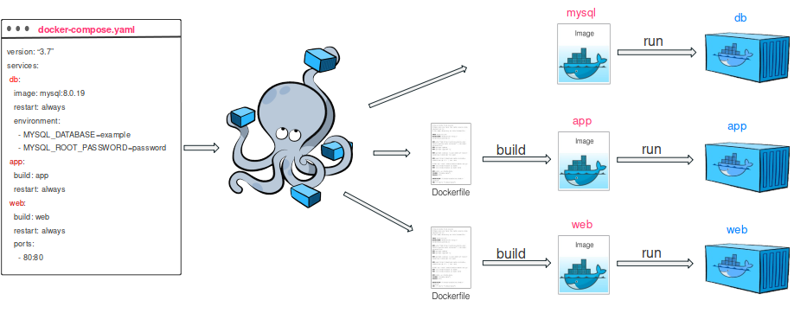
\includegraphics[width=0.4\linewidth]{compose.png}
\end{figure}

Tenéis muchos ejemplos en: \url{https://github.com/docker/awesome-compose/tree/master}
    
\end{frame}



\end{document}